\documentclass[11pt,letterpaper,titlepage]{article}
\usepackage[utf8]{inputenc}
\usepackage[T1]{fontenc}
\usepackage{amsmath}
\usepackage{amsfonts}
\usepackage{amssymb}
\usepackage{graphicx}
\usepackage{float}
\graphicspath{{./Images/}}

\title{Transient Electron Dynamics Simulator}

\begin{document}
	\begin{titlepage}
		\begin{center}
			\makeatletter
			{\huge \@title}
			\begin{large}
				\par User Manual
				\par v 1.2.
				\par "Layers"
			\end{large}
		\end{center}
		\makeatother
	\end{titlepage}
	
	\tableofcontents
	\newpage
	\section{Introduction}
		\par
		The Transient Electron Dynamics Simulator (TEDs) was originally designed to model a collection of time-dependent behaviors undergone by excited charge carriers within a nanowire with specified properties. Using a solver library like Scipy Integrate to evolve initial carrier distributions forward in time, the systems of differential equations can be solved numerically with a relatively simple Python script.
		
		\par
		Not so simple, however, is adapting a single Python solver for many nanosystem variants. Editing parameters directly in source code requires relaunching the solver repeatedly. Manually constructing initial distributions is tedious. Any solver can get the job done, but a solver operating underneath the hood of a graphical interface opens many opportunities for utility features to the solver and restores some user friendliness by minimizing the need to interact directly with source code.
		
		\par
		With that in mind, the goals of TEDs are to streamline how initial conditions and parameters are fed into the solver and offer more options for how to package the output of the solver. This we refer to as the initial state-simulation-data analysis workflow - a common pattern for many time-resolved finite-element problems.
		
		\par
		TEDs has since expanded beyond the single problem it was originally designed for. To maximize re-usability of TEDs, any problem is defined as a standalone module file, a recipe detailing the parameters TEDs needs to apply, the distinct physical layers TEDs should track, the outputs TEDs needs to calculate, and any special instructions TEDs needs to observe. New and existing module files may be swapped in and out as needed.
		
	\newpage
	\section{Getting Started}
		\subsection{Choosing a Simulation Model}
		\par
		When TEDs is launched, a Module Selection window appears:
		\begin{figure}[H]
			\label{fig:mod_select}
			\centering
			\includegraphics[scale=1]{"mod_select"}
			\caption{Three modules are available by default: a general-purpose one-layer material, a nanowire with axial rather than surface emission, and a specialized MAPI + Rubrene/DBP two-layer material.}
		\end{figure}
	
		\par
		TEDs scans the Modules directory for available module files and lists them in the Module Selection window. After selecting a module, TEDs performs some verification to ensure that the basic features of the module are correctly implemented, with all issues printed to console. This verification step does \textit{not} check the accuracy of or detect problems in more advanced features, such as custom module functions, but TEDS will report any issues with these features at the time they are invoked. After verification, TEDs then checks for the presence of a set of working directories – “Initial”, “Data”, and “Analysis” – and automatically creates these in the same directory as the source code if they are missing. TEDs also checks for and creates a subdirectory within “Data” for the specific module being loaded.
	
		\par
		It is \textit{highly recommended} that all files created by TEDs remain in these directories – they are the only places TEDs will search for files, and TEDs may not be able to locate files stored elsewhere.
		
		\subsection{Familiarizing with the Layout}
		
		\par
		After choosing a module, an interface like the following is displayed:
		\begin{figure}[H]
			\label{fig:main_interface}
			\centering
			\includegraphics[scale=0.4]{"main_interface"}
			\caption{Main interface.}
		\end{figure}
	
	    \par
	    The top left corner contains a menu containing options to close the program, toggle fullscreen view, change the active module, and open various utility features not contained in the main interface.
	    
	    \begin{figure}[H]
	    	\label{fig:top_left_menu}
	    	\centering
	    	\includegraphics[scale=1]{"top_left_menu"}
	    	\caption{Main menu.}
	    \end{figure}
	    
	    \par
	    The top left corner also contains three tabs — Inputs, Simulate, and Analyze, which correspond to the three main simulation stages of preparing an initial condition and parameter set, simulating the evolution of the initial condition over time, and viewing and analyzing the results. Each of the sub-interfaces displayed by these tabs are described in the following sections.
	    
	\newpage
	\section{The Inputs Tab - Defining the Model System}
		\subsection{Overview}
		    \par
		    One of the most powerful features of TEDS is the ability to construct spatial distributions of \textit{system parameters} in addition to \textit{initial conditions}, allowing models whose properties differ positionally to be simulated with no more difficulty than homogeneous models. The first step of creating a model is to define a space grid - wherein TEDs partitions the model length into equally sized nodes of specified width. Each node center and node edge may then take on its own set of values independent of the others. These collections of values are then saved as model state files and later read by the simulator.
			\par
			The Inputs Tab contains the following major components:
			
			\begin{figure}[H]
				\label{fig:labeled_main_interface}
				\centering
				\includegraphics[scale=0.4]{"labeled_main_interface"}
				\caption{Key parts of Inputs Tab.}
			\end{figure}
		
			\begin{enumerate}
				\item Initial Condition Subtabs 
				\par The Inputs Tab itself contains three subtabs – Laser Generation Condition, Parameter Toolkit, and Parameter List Upload. While initial condition and parameter distributions are zero by default, these three subtabs correspond to three methods available to modify them. A choice of subtab here affects the layout presented in [9].
				
				\item Save, Load, and Reset Buttons
				\par The Save and Load buttons are used to import and export model state files, discussed further in the sections \textit{Importing Model State Files} and \textit{Exporting Model State Files.}
				\par The Reset button clears specified system parameters and initial condition distributions from the interface and from the nodes, depending on the selected options, and is useful for correcting mistakes or restarting the model from a clean slate. Note that this feature does not affect the contents of previously saved model state files.
				
				\item Space Grid Entry Area
				\par Prior to entering node values, the space discretization grid for the model must first be established. The very first step of creating an model state file is entering the total length and node width (dx) here.
				\begin{figure}[H]
					\label{fig:locked_in_spacegrid}
					\centering
					\includegraphics[scale=1]{"locked_in_spacegrid"}
					\caption{A "locked in" space grid of length 1000 nm and node width 5 nm. This grid consists of 200 nodes whose centers are at 2.5, 7.5, 12.5...997.5 nm and whose edges are at 0, 5, 10...1000 nm.}
				\end{figure}
				
				\par Once any node value is assigned, the space grid becomes “locked in.” To enter a new space grid, clear the existing space grid using the “Clear All” option in the Reset button window.
				
				\item Fast Parameter Entry Tool
				
				\par Oftentimes, parameters will be constant throughout the entire system. This tool can be used to enter constant valued parameters quickly, while other tools should be used for more detailed distributions.
				
				\begin{figure}[H]
					\label{fig:fast_param_entry_tool}
					\centering
					\includegraphics[scale=0.7]{"fast_param_entry_tool"}
					\caption{Example list of values for each of the standard one-layer model's parameters. When "Continue" is clicked, all nodes and edges are assigned these values.}
				\end{figure}
			
				\par Parameters may be entered as numbers – e.g. 100, 9999, or 0.25 – or in scientific notation – e.g. 1e2, 9.999e3, 2.5e-1
				
				\item Flags Area
				
				\begin{figure}[H]
					\label{fig:flags}
					\centering
					\includegraphics[scale=1.5]{"flags"}
					\caption{Flags for the One-Layer module.}
				\end{figure}
				
				\par Module-specific flags can be toggled here. By default, each of the three included modules has two flags.
				
				\par The "Ignore Photon Recycle" flag deactivates carrier regeneration and photon recycling effects within the simulation. If these effects are known to be minor, neglecting these terms can speed up the simulation.
				
				\par The "Include FRET" flag determines whether fretting is active in the MAPI-Rubrene/DBP simulation. As with the "Ignore Photon Recycle" flag, this can be deactivated for a speedup if fretting is negligible.
				
				\par The "Steady State Input" flag alters how the initial carrier densities $\Delta N$ and $\Delta P$ are treated. When active, TEDs assumes that continuously, $\Delta N$ and $\Delta P$ carriers per $ nm^{-3}$ are added to the model per $ ns $. This also alters how the Laser Generation Condition works - the LGC calculates a carrier injection rate $ (\frac{carriers}{nm^{3} ns})$ rather than an initial carrier density distribution $(\frac{carriers}{nm^{3}})$ as from a single laser pulse.
				
				\par Furthermore, the Nanowire module defines an always-active hidden “symmetric system” flag – as according to its experimental setup (i.e. the Nanowire is excited at its center whereas the one-layer is excited at its surface). Any module, (including user-made ones) which includes this flag will, when this flag is activated for a model of length $L$, calculate a mirror model over the range 0 to $-L$ by copying the values from the actual model spanning 0 to $L$. This primarily affects whether photon recycle effects from the mirror space are included and whether integration into the mirror space is allowed.
				
				\item Status Box
				\par
				This box displays status and error messages associated with managing the model state.
				
				\item Model Summary Buttons
				\par These buttons can be used to view a list or plots of the current parameter values and can be used to verify a model state before saving to a file.
				
				\item Layer Selection Window
				\par This area is used to swap between a module's layers. Following their namesakes, the OneLayer and Nanowire modules feature one layer while the MAPI-Rubrene/DBP module features one each for MAPI and Rubrene/DBP.
				
				\par Each layer maintains its own space grid and set of parameters. Check which layer is currently active in the status box to ensure that changes are being made to the correct layer.
				
				\item Parameter Distribution Generation Suite
				\par The layout of this area and options available changes depending on which tab of [1] is selected. Details regarding how each of the generation suites operate are available in the subsections \textit{Laser Generation Conditions, Parameter Toolkit,} and \textit{Parameter List Upload}.
				
				\item Plots
				\par Each plot appearing in this area presents a visualization of recently updated parameters of the initial state.
				
				\par Toolbars below offer resizing and scaling of the Initial State Plots as well as options to export images of the plots.
				
			\end{enumerate}
		
			\subsection {Laser Generation Conditions (LGC)}
			\begin{figure}[H]
				\label{fig:LGC_blank}
				\centering
				\includegraphics[scale=0.5]{"LGC_blank"}
				\caption{Laser Generation Condition Tab.}
			\end{figure}
		
			\par For select modules, the Laser Generation Condition can be used to generate $\Delta N$ and $\Delta P$ according to a series of laser pulse excitation equations.
			
			\par Using the laser parameters shown above, this mode assigns values to $\Delta N$ and $\Delta P$ at each node for the selected layer using the following equations:
	
			\par First, the absorption coefficient $\alpha$ may be calculated from the below or entered directly.
			
			\begin{equation}
				\label{eq:LGC_absorption}
				\alpha = A_{0}\left(\frac{hc}{\lambda} - E_{g}\right)^{\gamma}
			\end{equation}
		
			\par The laser pulse profile may then be generated from one of four equation forms:
			
			\begin{equation}
				\label{eq:LGC_power}
				\Delta N(z) = \Delta P(z) = \frac{W}{Af\left(\frac{hc}{\lambda}\right)} \alpha e^{-\alpha z}
			\end{equation}
		
			\begin{equation}
				\label{eq:LGC_powerdensity}
				\Delta N(z) = \Delta P(z) = \frac{w''}{f\left(\frac{hc}{\lambda}\right)} \alpha e^{-\alpha z}, w''=\frac{W}{A}
			\end{equation}
		
			\begin{equation}
				\label{eq:LGC_maxgen}
				\Delta N(z) = \Delta P(z) = G_{max} e^{-\alpha z}
			\end{equation}
		
			\begin{equation}
				\label{eq:LGC_avggen}
				\Delta N(z) = \Delta P(z) = G_{avg}L\frac{\alpha e^{-\alpha L}}{e^{-\alpha z}\left(e^{-\alpha L} - 1 \right)}
			\end{equation}
		
			\par TEDs automatically performs all unit conversions needed to obtain $\Delta N$ and $\Delta P$ in $\frac{carriers}{nm^{3}}$ from values inputted in the listed units.
			
			\subsection{Parameter Toolkit}
			\par The Parameter Toolkit offers a fast, versatile way to sketch initial condition profiles by inputting a list of mathematical rules. Key parts of this interface are: 
			\begin{figure}[H]
				\label{fig:param_toolkit}
				\centering
				\includegraphics[scale=0.5]{"param_toolkit"}
				\caption{Parameter toolkit with one rule entered for parameter $\mu_{n}$. This rule, for example, assigns the value $10^{-5} \frac{cm^{2}}{V s}$ to all nodes spanning 0 nm to 100 nm.}
			\end{figure}
			\begin{enumerate}
				\item Rule List Window
				\par When a new parameter rule is added, a brief description of it will be added to this window. TEDs applies each of these rules one at a time, in order from top to bottom, to construct space distributions for the indicated parameter. Only one parameter’s rules are displayed at a time – see [3] for changing which parameter is displayed.
				
				\item Reordering Buttons
				\par Rules in [1] can be selected with a click and can be reordered in the list using these buttons. The order of which rules appear in the list is the order in which TEDs will apply them to the distribution - be sure to view the plots to ensure that the distribution is constructed as desired.
				
				\item Parameter Selection
				\par Select a parameter using the drop-down menu and click “Change view” to display that parameter’s rule list in [1]. This can also be used to change which parameter is plotted in the “Snapshot” plot.
				
				\item Rule Input Boxes
				\par These items are used to, for a new rule, specify the parameter for which it should be applied, the mathematical method used to apply it, and the values that the method should use. There are four mathematical methods – POINT, FILL, LINE, and EXP, and each of these are discussed in the following section \textit{Parameter Toolkit Mathematical Methods.}
				
				\item Deletion Buttons
				\par These buttons are used to delete either the selected rule or clear all rules for the currently displayed parameter.
			\end{enumerate}
		
		\subsection{Parameter Toolkit Mathematical Methods}
		\par Four mathematical methods are available for the parameter toolkit – POINT, FILL, LINE, and EXP.
		
		\par The POINT method is by far the most straightforward, assigning the Left Bound Value to the selected parameter’s initial distribution at the location specified by Left Bound Coordinate. Generally this refers to the single node containing that location, so the resolution of this method is specified by the node width. In the following example, this method is applied twice to create a very pointy $\Delta P$ initial distribution.
		
		\begin{figure}[H]
			\label{fig:ptoolkit_point}
			\centering
			\includegraphics[scale=1]{"ptoolkit_point"}
		\end{figure}
		\begin{figure}[H]
			\label{fig:ptoolkit_point_plot}
			\centering
			\includegraphics[scale=1]{"ptoolkit_point_plot"}
			\caption{In this example with the Nanowire module, the symmetric system flag is active - note the mirrored half of the system represented in the plot.}
		\end{figure}
	
		\par The FILL method fills every space point from the Left Bound Coordinate to the Right Bound Coordinate with the Left Bound Value. This method is useful for specifying regions with constant values and is a special case of the LINE method.
		
		\begin{figure}[H]
			\label{fig:ptoolkit_fill}
			\centering
			\includegraphics[scale=1]{"ptoolkit_fill"}
		\end{figure}
		\begin{figure}[H]
			\label{fig:ptoolkit_fill_plot}
			\centering
			\includegraphics[scale=1]{"ptoolkit_fill_plot"}
			\caption{In this example, three FILL commands are used to create a staircase-shaped distribution.}
		\end{figure}
		
		\par The LINE method assigns the Left Bound Value to the Left Bound Coordinate, assigns the Right Bound Value to the Right Bound Coordinate, and performs linear interpolation to assign values to all intermediate space points. Each intermediate point differs from its neighbors by a common difference value.
		
		\begin{figure}[H]
			\label{fig:ptoolkit_line}
			\centering
			\includegraphics[scale=1]{"ptoolkit_line"}
		\end{figure}
		\begin{figure}[H]
			\label{fig:ptoolkit_line_plot}
			\centering
			\includegraphics[scale=1]{"ptoolkit_line_plot"}
			\caption{In this example, the LINE command is used to draw a distribution from (0 nm, 1) to (100 nm, 10).}
		\end{figure}
		
		\par The EXP method is similar to LINE, but intermediate space points are instead filled by exponential interpolation between the left and right bounds. Each intermediate point differs from its neighbors by a common ratio.
		
		\begin{figure}[H]
			\label{fig:ptoolkit_exp}
			\centering
			\includegraphics[scale=1]{"ptoolkit_exp"}
		\end{figure}
		\begin{figure}[H]
			\label{fig:ptoolkit_exp_plot}
			\centering
			\includegraphics[scale=1]{"ptoolkit_exp_plot"}
			\caption{"In this example, an exponential curve is drawn from (0 nm, 100 000) to (80 nm, 10). The remaining space from 80 to 100 nm has value zero.}
		\end{figure}
		
		\par These four methods can be combined to set up complex distributions.
		
		\begin{figure}[H]
			\label{fig:ptoolkit_mixed}
			\centering
			\includegraphics[scale=1]{"ptoolkit_mixed"}
		\end{figure}
		\begin{figure}[H]
			\label{fig:ptoolkit_mixed_plot}
			\centering
			\includegraphics[scale=1]{"ptoolkit_mixed_plot"}
			\caption{LINE and FILL methods combined to create a "sawtooth" distribution.}
		\end{figure}
	
		\newpage
		\subsection{Parameter List Upload}
		\par Finally, TEDs can accept custom distributions in the form of .txt files containing lists of space coordinate and value pairs and apply these to a selected variable. Any space coordinates between those specified in the file will be filled in by linear interpolation. These .txt files must be formatted as two tab-separated columns, with the first column for coordinates and the second column for values
		
		\begin{figure}[H]
			\label{fig:listupload_blank}
			\centering
			\includegraphics[scale=1]{"listupload_blank"}
			\caption{List upload tab.}
		\end{figure}
	
		\par In the following example, the file “points.txt” is applied to $\Delta N$ over the range z=0 nm to z=6000 nm.
		
		\begin{figure}[H]
			\label{fig:listupload_example}
			\centering
			\includegraphics[scale=1]{"listupload_example"}
			\caption{Copying data from a spreadsheet program such as Excel can automatically provide the necessary tab-separated format.}
		\end{figure}
		
		\begin{figure}[H]
			\label{fig:listupload_example_plot}
			\centering
			\includegraphics[scale=1]{"listupload_example_plot"}
			\caption{The data are then linear interpolated to produce a bumpy-looking distribution on a log-scale plot up to 6000 nm, the final point in the file.}
		\end{figure}
	
		\subsection{Saving and Loading Model State Files}
		
		\par Before TEDs can simulate from initial distributions and system parameter sets, these must be saved as model state files (MSFs) using the “Save” feature.
		
		\begin{figure}[H]
			\label{fig:save_menu}
			\centering
			\includegraphics[scale=1]{"save_menu"}
			\caption{Also included is a debug button - this prints out log messages but serves no other function.}
		\end{figure}
	
		\par Once all system parameters have been entered, clicking the “Save” button will allow you to create and name a new model state file. MSFs have a specific layout designed to inform TEDs of where different items are located in the file.
		
		\par Saving an MSF without all system parameters entered is possible. In that case, all of the distributions would be saved as their default values – zeroes.
		
		\subsection{The Batch MSF Tool}
		
		\par In many situations, such as sensitivity analyses, it is useful to generate many model state files over a rectangular parameter space. In the “Tools” menu, TEDs offers the Batch Model State File Tool, which provides a fast method to generate many such copies based on an existing initial state.
		
		\begin{figure}[H]
			\label{fig:save_menu}
			\centering
			\includegraphics[scale=1]{"batch_blank"}
			\caption{Batch MSF Tool when first opened.}
		\end{figure}
	
		\par In the following example, the Batch MSF Tool is used to generate copies of “2-9-21.txt” from \textit{Saving and Loading Initial Conditions} with varying values of the parameter $\tau_{N}$: 10, 25, 40, 100, 1 000, and 10 000.
	
		\begin{figure}[H]
			\label{fig:batch_example}
			\centering
			\includegraphics[scale=1]{"batch_example"}
			\caption{Batch tool with example values entered.}
		\end{figure}
	
		\par When “Create Batch” is clicked, a directory is created within the Initial Directory, alongside any existing MSFs. Each file in the batch is procedurally named using the values of the varied parameters it has adopted.
		
		\begin{figure}[H]
			\label{fig:batch_example_dir}
			\centering
			\includegraphics[scale=0.9]{"batch_example_dir"}
			\caption{Resulting batch of MSF files.}
		\end{figure}
	
		\par Up to four parameters may be varied at a time.
		
		\subsection{Removing Files}
		
		\par In the top left corner menu under “File”, TEDs provides a series of shortcuts to each of the working directories.
		
		\begin{figure}[H]
			\label{fig:file_menu}
			\centering
			\includegraphics[scale=1]{"file_menu"}
			\caption{Clicking the File menu reveals various management options for the overall program.}
		\end{figure}
	
		\par Each of these opens the corresponding working directory, from where any files created by TEDs can be deleted.
		
	\newpage
	\section{Running Simulations}
	
	\par The Simulate tab contains the following major components:
	
	\begin{figure}[H]
		\label{fig:simulate_overview}
		\centering
		\includegraphics[scale=0.6]{"simulate_overview"}
		\caption{Key features of the Simulate Tab.}
	\end{figure}
	
	\begin{enumerate}
		\item Simulation Parameters
		
		\par This area contains input boxes in which the total time over which the system should be modeled and the time step size (dt) into which this total should be partitioned. Options to modify the behavior of the simulation, such as  module-specific flags, are specified per MSF in the Initial tab.
		
		\par There is also an input box to set the maximum time stepsize taken by solvers such as ODEINT. If left blank, by default the solver attempts to select an optimal internal stepsize to maximize speed while interpolating the data to the actual requested stepsize. However, sometimes this affects the accuracy of the solutions. If more accuracy is desired, a maximum stepsize can be specified here.
		
		\par For general cases, the recommended dt and solver stepsizes are shown above.
		
		\item Calculate Button
		\par When this button is clicked, a prompt opens for selecting previously saved MSFs. Multiple files may be selected and TEDs will simulate each of these in series with the settings in [1].
		
		\par When a simulation is complete, TEDs will create a folder  containing the results of the simulation in the corresponding module subdirectory within the “Data” directory. The name of this folder is based on the name of the MSF used to run the simulation.
		
		\item Status Window
		\par Like its counterpart in the inputs tab, this window displays status messages and problems encountered when performing the simulations.
		
		\item Results Windows
		\par These plots display snapshots of time steps taken during the simulation, a useful first glance of how the model is evolving over time. As with the Initial tab plots, these plots have a toolbar for basic resizing and exporting. 
		
	\end{enumerate}

	\newpage
	\section{Analyzing and Integrating Simulation Data}
		\par The Analyze tab contains two subtabs – Overview and Detailed Analysis.
		
		\par The Overview tab plots a snapshot of various outputs over time for a selected data folder. For the One-Layer and Nanowire modules, these are, in addition to $\Delta N$ and $\Delta P$: the internal electric field, nonradiative and radiative combination, TRPL over full thickness, and effective lifetime $\tau_{diff}$
		
		\begin{figure}[H]
			\label{fig:overview_blank}
			\centering
			\includegraphics[scale=0.36]{"overview_blank"}
			\caption{The Overview subtab when first opened. Click "Select Dataset" to choose a data set.}
		\end{figure}
	
		\begin{figure}[H]
			\label{fig:overview_example}
			\centering
			\includegraphics[scale=0.36]{"overview_example"}
			\caption{An example overview of a MAPI/Rubrene-DBP data set.}
		\end{figure}
	
		\par Two types of plots are displayed - plots which display selected timesteps over the space grid and plots which display values calculated over the time grid. The "No. Samples" box and adjacent log/linear selector determine which timesteps are selected.
		
		\par To view other timesteps or TRPL over other ranges, for example, the Detailed Analysis tab should be used.
		
		\par The Detailed Analysis tab contains four smaller plots – for navigating through the time steps of selected data sets, and one larger plot – for showing results from integrating data sets from the smaller plots.
		
		\par The defining feature of this tab is that each plot is equipped with a more detailed toolbar, each feature of which is covered in the following sections.
		
		\begin{figure}[H]
			\label{fig:detailed_example}
			\centering
			\includegraphics[scale=1]{"detailed_example"}
			\caption{An example of the Detailed Analysis tab in use. Here the TRPL data of three datasets is compared.}
		\end{figure}
		
		\begin{figure}[H]
			\label{fig:detailed_toolbar}
			\centering
			\includegraphics[scale=1]{"detailed_toolbar"}
			\caption {Toolbar for analysis plots.}
		\end{figure}
	
		\subsection{Plotting}
		
		\par The “Plot” button opens the following popup, from which there are options to select which variable should be plotted on the y-axis and which data sets should be plotted.
		
		\begin{figure}[H]
			\label{fig:plotting_example}
			\centering
			\includegraphics[scale=1]{"plotting_example"}
			\caption{To select a single dataset, click its name in the box. 
			To select multiple datasets, hold the Ctrl key and drag the cursor over every desired dataset.
			}
		\end{figure}
	
		\par When “Continue and select datasets” is clicked, the first time step of each selected dataset (i.e. the initial condition) is plotted. If the “Auto Integrate All Time and Space Steps” option is selected, TEDs will also integrate all time steps over the full length of the system and display the result in the large plot.
		
		\begin{figure}[H]
			\label{fig:analyze_example}
			\centering
			\includegraphics[scale=1]{"analyze_example"}
			\caption{PL data from the previously selected data sets. All data when first plotted show their initial t=0 values.}
		\end{figure}
	
		\par One limitation, as demonstrated above by the fact that only four of the seven selected datasets have been plotted, is that the plotter can only plot datasets together if they have the same total time and time step size. If datasets with different total time or time step size should be compared, plotting each on a different plot is recommended.
		
		\par Datasets with different space grids and identical time grids, however, are compatible with one another.
		
		\subsection{Stepping Through Time}
		\par Directly to the right of the “Plot” button is the “Step” input box and button. When the “Step” button is clicked, all plotted datasets are advanced by the number of time steps specified in the input box. How far ahead the datasets are advanced in absolute time depends on the size of the time steps used in the simulation.
		
		\par With a time step size of 0.5 ns, for example, entering 20 will advance the datasets by 10.0 ns. each time the “Step” button is clicked.
		
		\begin{figure}[H]
			\label{fig:step_forward_example}
			\centering
			\includegraphics[scale=1.0]{"step_forward_example"}
			\caption{Data sets at a later time.}
		\end{figure}
	
		\par Stepping with a negative number of time steps will cause TEDs to move the datasets \textit{backward} that many time steps.
		
		\subsection {Changing Axis Settings}
		
		\par The “Axis Settings” button opens a popup to change the lower bounds, upper bounds, and scaling type of the x and y axes. Options to toggle the legend visibility or freeze the axes are also available.
		
		\begin{figure}[H]
			\label{fig:axis_settings_example}
			\centering
			\includegraphics[scale=1.2]{"axis_settings_example"}
			\caption{Adjusting the x and y axes. When opened, the Axis Settings popup is populated with the current axis values.}
		\end{figure}
	
		\par TEDs will attempt to determine the best axis range and scale (linear or log) based on the values spanned by the data and will update the axes continuously as the displayed data is changed. Sometimes this does not work well, and other times static axes are preferred. In that case the “Freeze Axes” option can be used to fix and specify the axes manually.
		
		\subsection {Exporting Data}
		
		\par The “Export” button opens a prompt to save the currently plotted data to a .csv file, which can be viewed with Excel or any text editor. These files have an alternating column format – where x is the x-axis variable (position, time, or parameter value) and y is the y-axis variable, the first and second columns are the (x, y) data points of the first data set, the third and fourth columns are (x, y) for the second data set, and so on.
		
		\begin{figure}[H]
			\label{fig:export_example}
			\centering
			\includegraphics[scale=0.8]{"export_example"}
			\caption{Example exported .csv file viewed using Microsoft Excel.}
		\end{figure}
	
		\subsection {Regenerating MSFs from Existing Data}
		
		\par Finally, the “Generate IC” button opens a popup that can be used to construct a new MSF from previously simulated datasets.
		
		\begin{figure}[H]
			\label{fig:carryover_example}
			\centering
			\includegraphics[scale=1]{"carryover_example"}
			\caption{Example MSF regeneration popup based on the currently loaded data sets.}
		\end{figure}
	
		\par First, the checkboxes are used to indicate which variables should be copied into the new MSFs. For the one-layer and nanowire modules, $\Delta N$ and $\Delta P$ may be copied. The selection box, which functions like the “Plot” button’s, is then used to indicate which datasets MSFs should be generated for. When “Continue” is clicked, one MSF will be created with the selected variables for each dataset and prompts will appear to name the MSFs.
		
		\par These MSFs can then be modified further using the Initial tab or simulated using TEDs’ other tabs.
		
		\subsection {Integration}
		
		\par TEDs supports two integration modes – “Over Time”, which integrates the plotted variable over a specified space interval at all time steps and generates a plot of how the integrated variable evolves over time, and “Current Time Step”, which integrates over the space interval at only the currently displayed time step. Because time is not displayed on the horizontal axis in the “Current Time Step” mode, the user is free to assign any variable to this axis. Combined with the Batch Initial Condition Tool, the “Current Time Step” mode is useful for sensitivity analyses over single parameters.
		
		\par For example, we may want to examine how the carrier density near the front of a Nanowire is affected by the negative charge carrier mobility $\mu_N$, but a plot of the spatial distributions can be quite chaotic.
		\begin{figure}[H]
			\label{fig:mubatch_example}
			\centering
			\includegraphics{"mun"}
		\end{figure}
	
		\par An integral may summarize the differences more clearly. Upon clicking “Integrate”, the following popup appears for selecting the integration mode.
		
		\begin{figure}[H]
			\label{fig:integration_mode_example}
			\centering
			\includegraphics{"integration_mode_example"}
		\end{figure}
		
		\par When “Continue” is clicked, the next popup appears for specifying the lower and upper space boundaries of the integration.
		
		\begin{figure}[H]
			\label{fig:integration_getbounds_blank}
			\centering
			\includegraphics{"integration_getbounds_blank"}
		\end{figure}
	
		\par The “Single integral” option performs one integral per dataset over the specified bounds. The “Multiple integrals” performs a set of integrals per dataset, each at a specified centerpoint with given width. These integrals will be cut off at the boundaries if the centerpoint and width would normally take the integral past the boundaries. A system with length 10 000 nm, for instance, will stop integration at 10 000 nm regardless of inputs.
		
		\begin{figure}[H]
			\label{fig:integration_getbounds_example}
			\centering
			\includegraphics{"integration_getbounds_example"}
			\caption{In this example, integrals over [0,500], [500,1500], and [1500,2500] nm will be performed.}
			
		\end{figure}
		
		\par For systems with the “symmetric system” flag active during a simulation, the integration can pass into the symmetric “other half” – for example, Fig. ~\ref{fig:integration_getbounds_example} will instead span over [-500, 500], [500,1500], and [1500,2500].
		
		\par For simplicity we will examine a single integral by modifying the inputs from the example above. Note that the "Multiple Integrals" feature allows for single integrals too.
		
		\begin{figure}[H]
			\label{fig:integration_getbounds_example2}
			\centering
			\includegraphics[scale=0.77]{"integration_getbounds_example2"}
			\caption{In this example, one integral over [500,1500] nm will be performed.}
			
		\end{figure}
	
		\par If the “Current Time Step” mode is selected, a third popup will appear for selecting the variable to be plotted on the horizontal axis.
		
		\begin{figure}[H]
			\label{fig:integration_xaxis_example}
			\centering
			\includegraphics{"integration_xaxis_example"}
			\caption{The module parameters determine the available axes - in this case $\mu_{N}$ is selected because the data originate from MSFs with differing mobility values.}
		\end{figure}
	
		\par The following plot is generated, but adjusting the vertical axis using the “Axis Settings” should prove helpful.
		
		\begin{figure}[H]
			\label{fig:integration_result}
			\centering
			\includegraphics{"integration_result"}
		\end{figure}
	
		\begin{figure}[H]
			\label{fig:integration_result_adj}
			\centering
			\includegraphics{"integration_result_adj"}
			\caption{Integration results before and after adjusting using Axis Settings. As expected, high mobility allows negative charge carriers to reach this region of the Nanowire faster, but this effect is only visible when mobility is sufficient to put the diffusion timescale near 2 ns.}
		\end{figure}
	
		\subsection{Time Series - Extracting Additional Information from Integrated Data}
		
		\par When certain integrals are computed, TEDs will use the freshly integrated data to make additional calculations. TEDs calls these "Time Series" and displays the results in pop-up windows after the integration is complete.
		
		\begin{figure}[H]
			\label{fig:timeseries_example}
			\centering
			\includegraphics[scale=0.38]{"timeseries"}
			\caption{For example, when the TRPL over the MAPI layer of a MAPI-Rubrene/DBP dataset is computed, TEDs also computes the effective carrier lifetime and PL efficiency.}
		\end{figure}
	
		\par The following table summarizes the Time Series available for each module. Integrate the quantity in the left column to obtain the values in the right column.
		
		\begin{figure}[H]
			\label{fig:timeseries_table}
			\centering
			\includegraphics[scale=0.6]{"timeseries_table"}
		\end{figure}
	
	\newpage
	\section{Adding a Custom Module - Python Familiarity Recommended}
	
		\subsection{The Module Object Hierarchy}
	
		\begin{figure}[H]
			\label{fig:py_hierarchy}
			\centering
			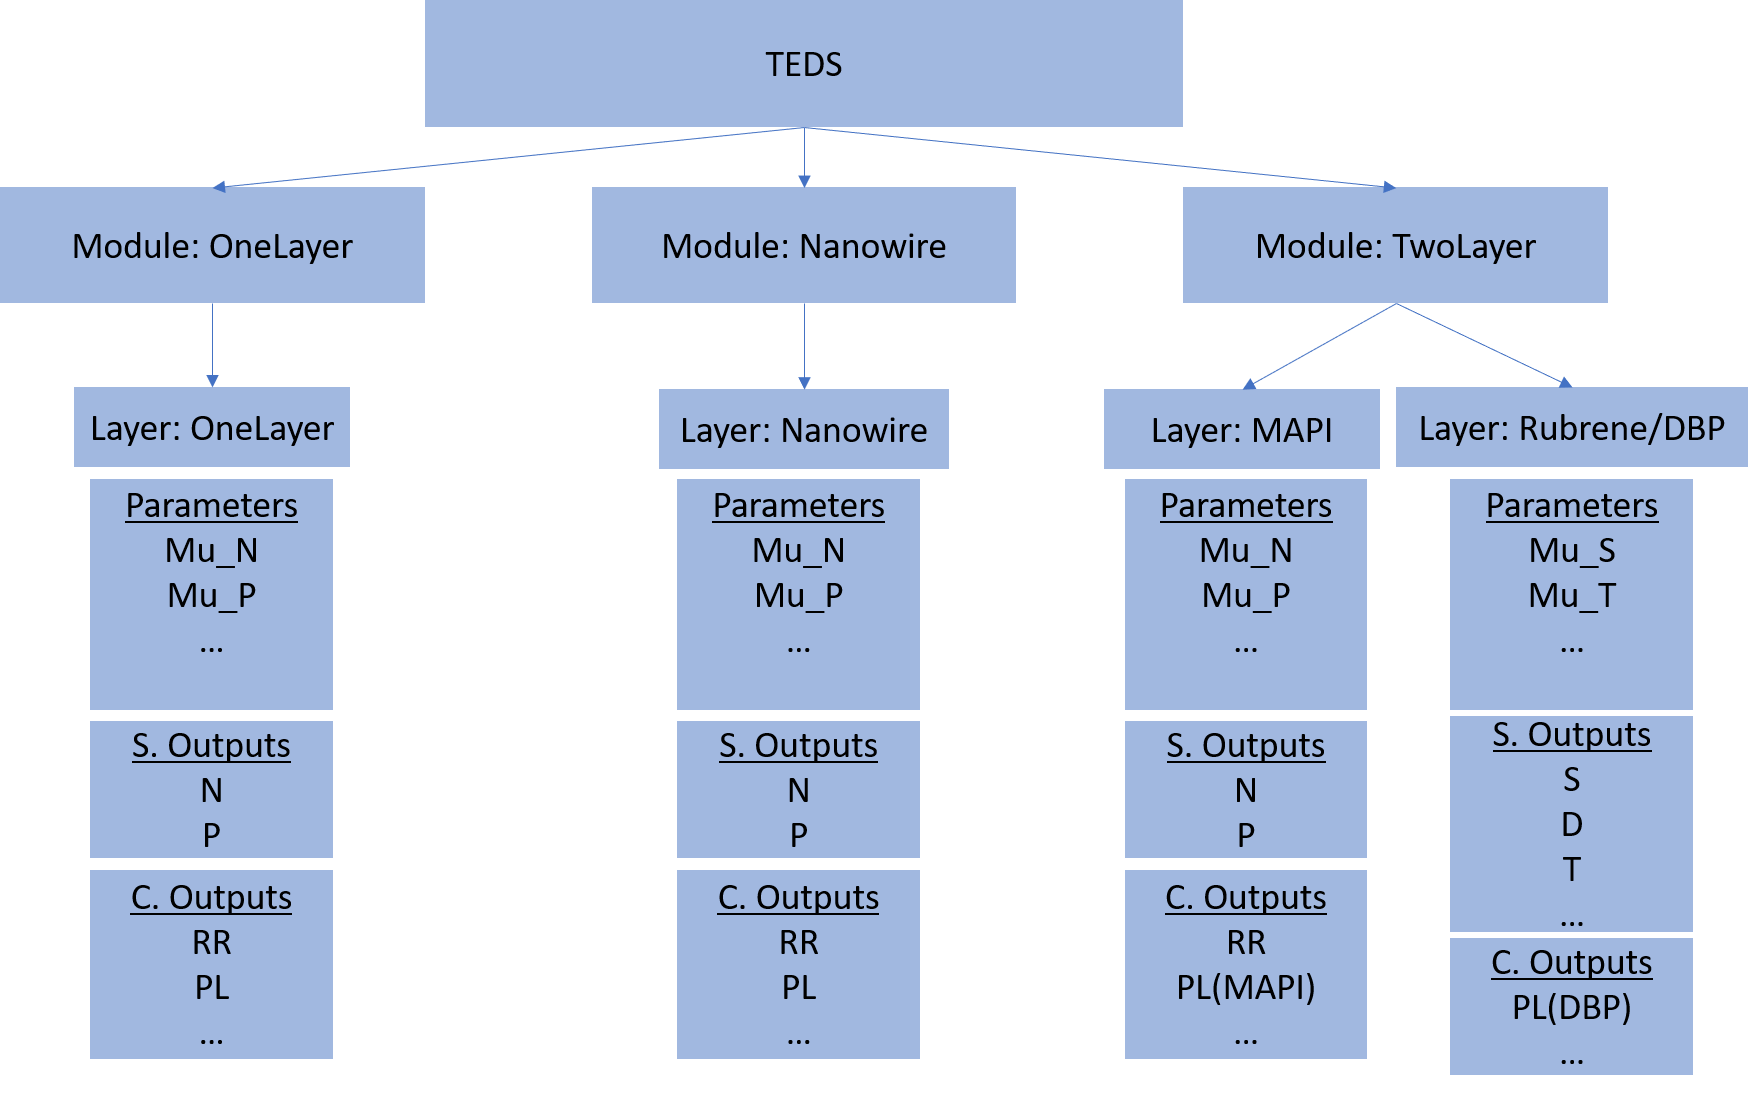
\includegraphics[scale=0.4]{py_object_hierarchy.png}
			\caption{Multilayer structure of TEDs modules.}
		\end{figure}
	
		\par The \textit{Layer} is the fundamental building block of a TEDs module, representing a self-contained physical system with defined parameters, inputs, and outputs. Parameters and outputs are themselves objects which track internal information such as their names, values, and whether they exist on node edges or centers. Layers manage these objects and may interact with other layers according to the functions packaged in the module.
		
		\subsection{Filling Out the Module Template}
		
		\par By extending the OneD\_Model template class in the file \_OneD\_Model.py, custom modules can be created and simulated with TEDs. A complete module.py file must implement the following functions with the exact arguments specified in the template:
		
		\begin{itemize}
			\item \_\_init\_\_()
			\item calc\_inits()
			\item simulate()
			\item get\_overview\_analysis()
			\item prep\_dataset()
			\item get\_timeseries()
			\item get\_IC\_carry()
		\end{itemize}
	
		\par Additionally, any functions used by a module for calculating values should be defined within that module file. It is highly recommended that these employ Numpy vectorization or similar for compatibility with both 1D and 2D inputs.
	
		\par Once complete, the module.py file must be placed into the Modules directory and imported into main.py. An entry must also be added into mod\_list() in main.py. The new module can then be selected when TEDs is started.
		
		\begin{figure}[H]
			\label{fig:modules_here}
			\centering
			\includegraphics[scale=0.9]{"modules_here"}
		\end{figure}
	
		\par The One-Layer module is the recommended starting point for semiconductor materials, while other modules demonstrate how more advanced behaviors may be incorporated.
		
		\subsubsection{\textunderscore\textunderscore init \textunderscore\textunderscore()}
		
		\par This function sets up all informational variables associated with the module and informs TEDs of what parameters or outputs need to be tracked for each layer. For the overall  \textbf{Module}, the following attributes must be implemented:
		
		\begin{itemize}
			\item system\_ID
			\par This is a string specifying the unique identifier of the module. Any string is acceptable, but it is recommended that the system\_ID reflect the name of the problem the module is intended to represent. For example, the standard One-Layer's system\_ID is "OneLayer".
			
			\item time\_unit
			\par This is a string specifying the time unit (e.g. "ns") the time grid is calculated in. This field is for plotting display purposes only (i.e. not explicitly used in calculations) but should match the internal time unit used by the module. For example, the time grid actually operates in units of ns for the three provided modules. User-created modules which describe slower physical phenomena may wish to design their solvers on the basis of larger time units.
			
			\item flags\_dict
			\par This dictionary can be used to define custom system flags, whether these values should be toggleable, and their default values. Examples of these are the "Steady State Input" and "Ignore Photon Recycle" flags described in the Initial Tab Overview section.
			
			\item layers
			\par This dictionary lists the Layer objects that a module is composed of. As discussed in the upcoming section, Layers control their own lists of parameters and outputs.
			
		\end{itemize}
	
		\subsubsection{Defining Layers}
		\par Layers are initialized with the following values:
		
		\begin{itemize}
			\item length\_unit
			\par This is a string specifying the length unit (e.g. "nm") the space grid for this layer is calculated in. Like the Module time\_unit, This field is for plotting display purposes only (i.e. not explicitly used in calculations) but should match the internal length unit used by the layer. For example, the space grid operates in units of nm for all layers in the three provided modules. Since the internal time unit is ns, this means all incoming parameters for these modules must be converted to the nm-ns unit system and all raw outputs will come out with these units. See the convert\_in and iconvert\_in sections for additional details.
			
			\item params
			\par This is a dictionary of Parameter objects corresponding to the parameters which exist in this layer. For example, in the MAPI-Rubrene/DBP module, the MAPI Layer contains parameter objects for N and P mobilities while the Rubrene Layer contains similar objects for T, S, and D mobilities. Both material properties, such as mobilities, and initial conditions, such as $\Delta N(t=0)$, should be defined here.
			
			\item simulation\_outputs
			\par This dictionary specifies outputs which are returned directly when TEDs simulates a system created from the module and uses Output() objects to store information regarding these outputs. For example, the One-Layer module simulates carrier densities; therefore the simulation outputs are $N(x,t)$ and $P(x,t)$. The display information is used to populate plot fields.
			
			\par Any output here should have a corresponding Parameter from which initial values may be calculated. For example, the Output $N$ has Parameters $\Delta N(t=0)$ and $N_0$ which together calculate $N(t=0)$.
			
			\item calculated\_outputs
			\par This dictionary specifies outputs which are calculated from those listed in simulation\_outputs but not simulated directly. For example, TRPL is not calculated during a simulation, but rather from $\Delta N$ and $\Delta P$ after the fact.
			
			\par simulation\_ and calculated\_outputs are also combined into a single outputs dictionary for convenience.
			
			\item convert\_in
			\par This dictionary specifies conversion factors that should be used to change from the units entered into the interface to the internal solver units. Generally, this dictionary should be used to correct mismatches between common length and time units (such as inputting $cm^{-3}$ for carrier densities) and the length and time scale used by the module (i.e. the space grid is in $nm$ and works with $N$ in units of $nm^{-3}$ rather than their $cm$ counterparts). One conversion factor must be defined for each Parameter and Output. Quantities which do not need conversions should be assigned a conversion factor of 1.
			
			\item iconvert\_in
			\par This dictionary specifies conversion factors that should be applied in addition to \textit{convert\_in} when integrals are calculated. For example, $N$ needs a \textit{convert\_in} entry to switch between $cm^{-3}$ and $nm^{-3}$, but when integrated over length, $N$ switches between $cm^{-2}$ and $nm^{-2}$ instead. The \textit{iconvert\_in} entry addresses the difference between $length^{-2}$ to $length^{-3}$. One conversion factor must be defined for each Output. Quantities which do not need conversions should be assigned a conversion factor of 1.
		\end{itemize}
	
		\subsubsection{Defining Parameters}
		\par Parameters are initialized with the following values:
		
		\begin{itemize}
			\item units
			\par This is a string specifying the units to be displayed with this parameter. Use this field to indicate the units this parameter should be entered and the conversion dictionaries to convert into internal solver units.
			
			\item is\_edge
			\par Whether this parameter should be assigned to space node centers or space node edges.
			
			\item valid\_range
			\par A tuple [a,b] used to restrict the allowed values for this parameter. Inputting values smaller than a or larger than b will raise an error. For example, only positive (a=0, b=infinity) mobility values are allowed. This is useful for screening out nonsense inputs.
			
			\item is\_space\_dependent
			\par Setting this flag to False will exclude this parameter from all input methods except for the Fast Parameter Entry Tool, effectively allowing only single values to be assigned to this parameter. Surface parameters, such as the front and back surface recombination velocities, should have this flag deactivated.
				
		\end{itemize}
	
		\subsection{calc\textunderscore inits()}
		\par This function is used by TEDs to obtain all initial conditions needed by the solver and must return a dictionary \{“param name”:np.ndarray\} containing one 1D array with the initial value of each space node per output in simulation\_outputs. Use of the module’s parameter dictionaries to access material parameter values, convert\_in for unit conversions, and grid\_x\_nodes, and/or grid\_x\_edges to access the space grids is highly recommended.
		
		\subsection{simulate()}
		\par This function is used by TEDs to call the function(s) responsible for (1) preprocessing inputs, (2) simulating the data, and (3) writing the data to output files. It is not required to use all of simulate()’s arguments, and any implementation which completes the three mentioned items is acceptable. For the One-Layer, all three of these tasks are completed by the driver function ode\_nanowire().
		
		\subsection{get\_overview\_analysis()}
		\par Like calc\_inits(), this function must return a dictionary \{“param name”:np.ndarray\} containing one array per output in simulation\_ and calculated\_outputs. The u\_read() helper function is recommended for reading in a section of data over a specified time and space range.
		
		\subsection{prep\_dataset()}
		\par This function is used to do preprocessing of data prior to plotting and must return a 1D array of data (a single time step) to be plotted or a 2D array (time and space) to be integrated. For instance, in some modules the TRPL requires multiplying the radiative recombination by a weighting function to account for photon recycling prior to plotting. For most outputs preprocessing is simply reading the appropriate entry of sim\_data or calling an appropriate calculation function.
		
		\subsection{get\_timeseries()}
		\par This function is used to calculate the time series associated with specific outputs. A list of tuples should be returned - one tuple per time series. Each tuple contains two values - first value the name of the time series and second value a 1D np.ndarray containing the time series values. 
		
		\subsection{get\_IC\_carry()}
		\par This function is used to assign current data values to param\_dict for regenerating MSF files using the carryover feature. This function must write into the appropriate entry of param\_dict using include\_flags to determine how to respond to which items are selected in the carryover feature.

\end{document}